\begin{frame}
\begin{center}
Speaking of useful operations\ldots
\end{center}
\end{frame}

\begin{frame}
\begin{block}{Comonad is}
Any functor \lstinline{F} supporting:
\begin{center}
\begin{itemize}
  \item<1-> \lstinline{extract :: F a -> a}
  \item<2-> \lstinline{duplicate :: F a -> F (F a)}
  \item<3-> \emph{satisfying laws of identity and associativity}
\end{itemize}
\end{center}
\end{block}
\end{frame}

\begin{frame}
\begin{center}
Does a \lstinline{ListZipper} satisfy the requirements for a comonad?
\end{center}
\end{frame}

\begin{frame}[fragile]
\begin{block}{Yes}
\begin{center}
\begin{lstlisting}[style=haskell]
fmap :: (a -> b) -> ListZipper a -> ListZipper b
extract :: ListZipper x -> x
duplicate :: ListZipper w -> ListZipper (ListZipper w)
\end{lstlisting}
\end{center}
\end{block}
\end{frame}

\begin{frame}
\begin{center}
What about a \lstinline{TreeZipper}?
\end{center}
\end{frame}

\begin{frame}[fragile]
\begin{block}{Yes}
\begin{center}
\begin{lstlisting}[style=haskell]
fmap :: (a -> b) -> TreeZipper a -> TreeZipper b
extract :: TreeZipper x -> x
duplicate :: TreeZipper w -> TreeZipper (TreeZipper w)
\end{lstlisting}
\end{center}
\end{block}
\end{frame}

\begin{frame}[fragile]
\begin{block}{Actually}
\begin{center}
\textbf{All} zippers are comonads \emph{(Uustalu, 2005)}
\end{center}
\end{block}
\end{frame}

\begin{frame}[fragile]
\begin{block}{Here is a utility function}
\begin{center}
\begin{lstlisting}[style=haskell]
-- Do any (max: 2) adjacent focii of the list zipper
-- satisfy the given predicate?
adjacentFociiSatisfy ::
  (a -> Bool)
  -> ListZipper a
  -> Bool
adjacentFociiSatisfy p z =
  let mvs k = any p (focus <$> k z)
  in  mvs moveLeft || mvs moveRight
\end{lstlisting}
\end{center}
\end{block}
\end{frame}

\begin{frame}[fragile]
\begin{block}{Requirement}
\begin{center}
Find all zippers with a focus adjacent to a given value
\end{center}
\end{block}
\end{frame}

\begin{frame}[fragile]
\begin{block}{Find all zippers with a focus adjacent to a given value}
\begin{itemize}
  \item<1-> \lstinline{duplicate}

            we now have \lstinline{ListZipper (ListZipper a)}
  \item<2-> \lstinline{toList}

            we now have \lstinline{[ListZipper a]}
  \item<3-> \lstinline{filter} with \lstinline{adjacentFociiSatisfy}

            we still have \lstinline{[ListZipper a]}
\end{itemize}
\end{block}
\end{frame}

\begin{frame}[fragile]
\begin{block}{\lstinline{allWithAdjacent}}
\begin{center}
\begin{lstlisting}[style=haskell]
allWithAdjacent ::
  Eq a =>
  a
  -> ListZipper a
  -> [ListZipper a]
allWithAdjacent n =
  filter (adjacentFociiSatisfy (==n)) . toList . duplicate
\end{lstlisting}
\end{center}
\end{block}
\end{frame}

\begin{frame}[fragile]
\begin{block}{\lstinline{allWithAdjacent}}
\begin{center}
\begin{lstlisting}[style=haskell]
> allWithAdjacent 3 (ListZipper [3,2,1] 4 [5..10])
[
  ListZipper {
    lefts = [1]
  , focus = 2
  , rights = [3,4,5,6,7,8,9,10]
  }
, ListZipper {
    lefts = [3,2,1]
  , focus = 4
  , rights = [5,6,7,8,9,10]
  }
]
\end{lstlisting}
\end{center}
\end{block}
\end{frame}

\begin{frame}[fragile]
\begin{block}{\lstinline{allWithAdjacent}}
\begin{center}
\begin{lstlisting}[style=haskell]
> allWithAdjacent 3 (ListZipper [3,2,1] 4 [7,2,6,3])
[
  ListZipper {
    lefts = [1]
  , focus = 2
  , rights = [3,4,7,2,6,3]
  }
, ListZipper {
    lefts = [3,2,1]
  , focus = 4
  , rights = [7,2,6,3]
  }
, ListZipper {
    lefts = [2,7,4,3,2,1]
  , focus = 6
  , rights = [3]
  }
]
\end{lstlisting}
\end{center}
\end{block}
\end{frame}

\begin{frame}
\begin{center}
Who's wanted that in their text editor before?
\end{center}
\end{frame}

\begin{frame}
\begin{center}
What were you editing? JSON? Your pilot logbook?
\end{center}
\end{frame}

\begin{frame}
\begin{center}
What about \textbf{a programming language}?
\end{center}
\end{frame}

% \begin{frame}
% \begin{center}
% I'll leave \lstinline{TreeZipper} comonad operations to your imagination
% \end{center}
% \end{frame}

\begin{frame}
\begin{block}{other uses of zippers}
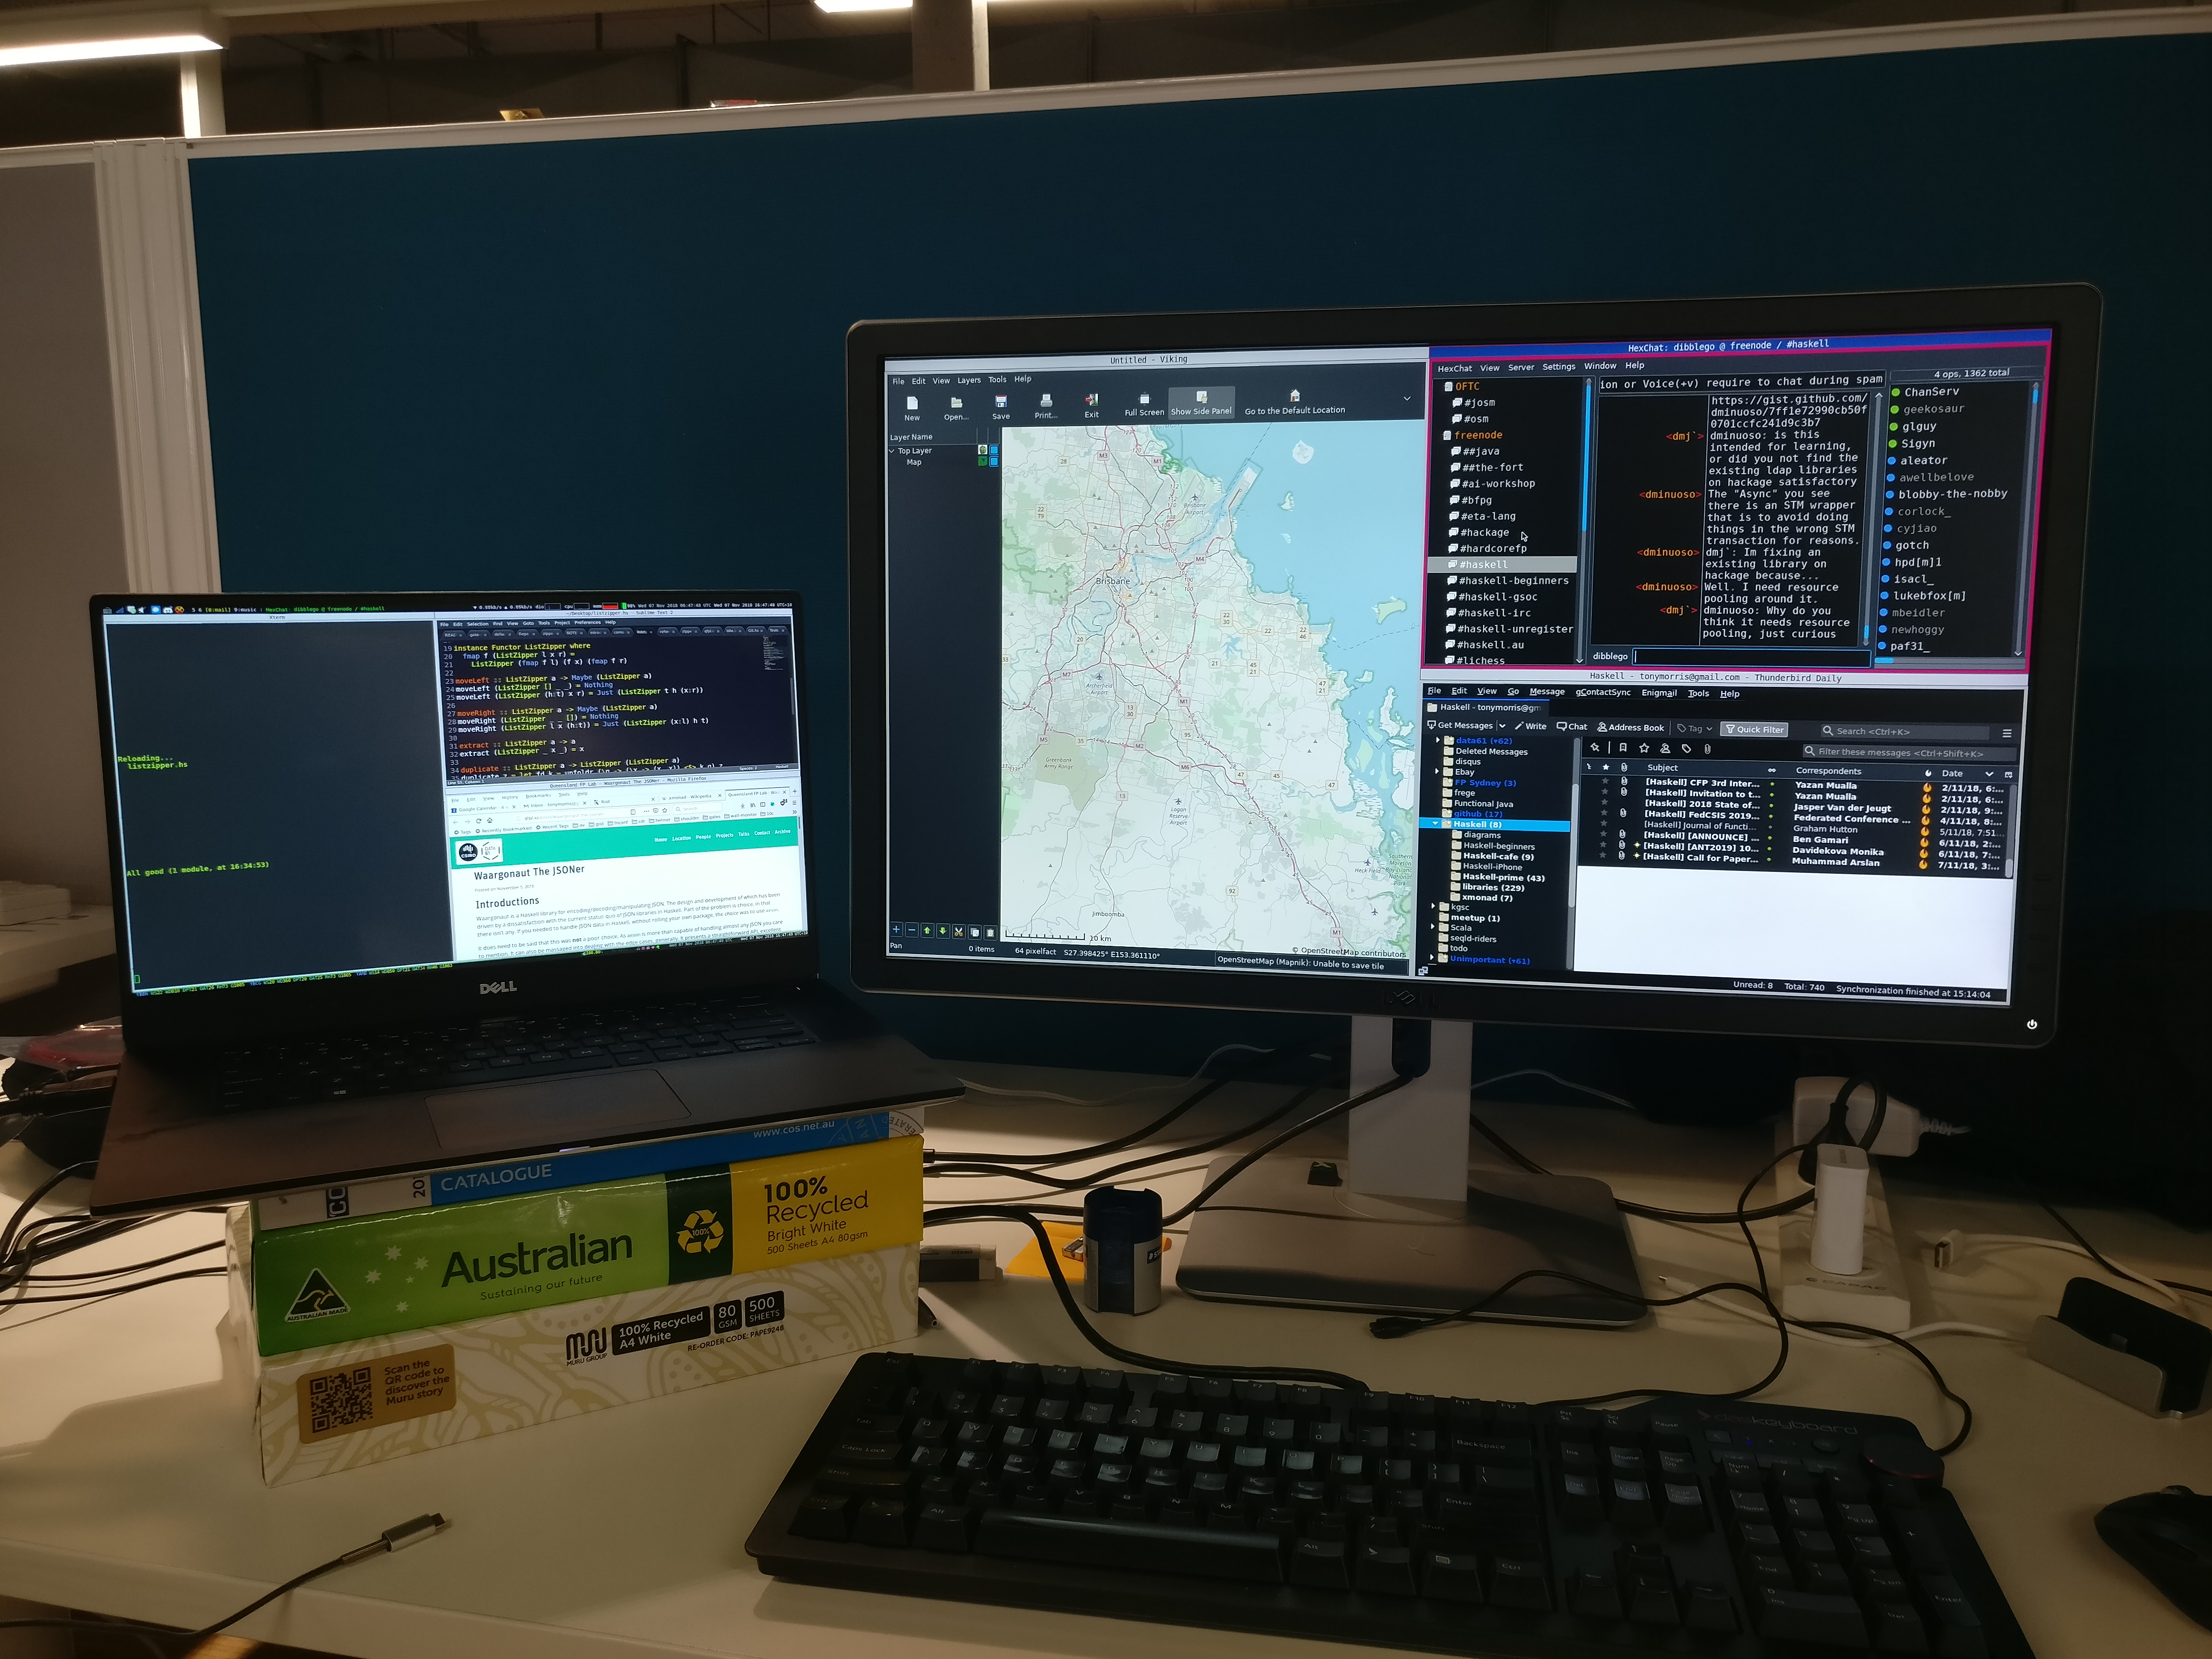
\includegraphics[width=1.00\textheight]{image/xmonad.jpg}
\end{block}
\end{frame}
